\Chapter{Gépi játékos megvalósítása}

Kíváncsi voltam, hogy létezik-e bizonyított stratégia a Monopoly játék megnyereséhez, ezért utánanéztem az interneten. Mi befolyásolhatja a minél jobb helyezést? Mire érdemes odafigyelni? Hogyan gazdálkodjak a pénzemmel? A talált cikkekben lévő információkat összegezve kialakultak azok a tényezők amiket érdemes megvizsgálni, a szimulációk során ezeket fogom paraméterezni. A cikkek hivatkozása az Irodalomjegyzékben megtalálható.


\Section{Szolgáltatók és bizniszek}

Matematikai mérésekkel igazolható, hogy a szolgáltatók megvásárlása pénzkidobás, hiszen mire megtérülne a befektetett összeg addigra már a játék késői szakaszában vagyunk, ahol általánosságban elmondható, hogy az itt szerezhető pénz elenyésző lenne a kiadásokhoz képest.

A bizniszekek azonban már nagyobb pénzszerzési lehetőséget biztosítanak a játék korai, illetve középső szakaszában, később a jelentőségük pedig elhanyagolható.

\newpage
\Section{Telkek és fejlesztései}

Többen is vizsgálták, hogy a telkek elhelyezkedésének a játéktáblán és árának, illetve annak megtérülési idejének milyen jelentősége lehet. Az ehhez készült grafikon:

\begin{figure}[h!]
\centering
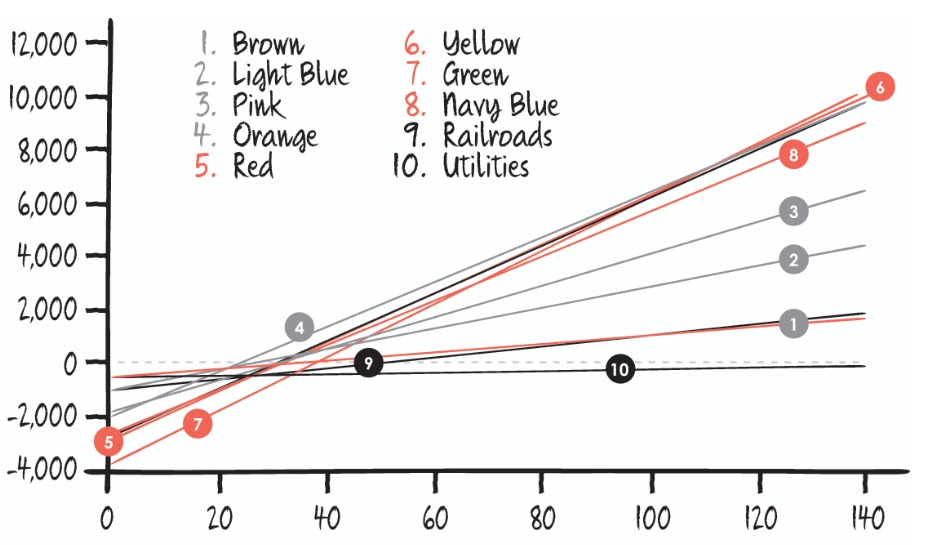
\includegraphics[scale=0.4]{images/monop1.jpg}
\caption{1. Barna 2. Világoskék 3. Rózsaszín 4. Narancs 5.Piros 6. Sárga 7. Zöld 8. Sötétkék 9. Biznisz 10. Szolgáltató
Forrás: https://g7.hu/elet/20180506/ezzel-a-taktikaval-hamar-nyomorba-dontod-a-jatekostarsaidat-monopolyban/}
\label{fig:ff}
\end{figure}

Arra jutottak, hogy a börtön után lévő telkekre éri meg leginkább összpontosítani. A fejlesztéseket tekintve több stratégia is szóba jött, ezeknek a lényege leginkább, hogy kiszorítsuk versenytársainkat a piacról azzal, hogy felvásároljuk előttük az összes fejlesztést, így kevesebb hozamot szereznek. Ennek mértéke váltakozó, van olyan állítás is, miszerint 3 fejlesztésnél álljunk meg, viszont akad olyan is ami szerint 4 fejlesztés az ideális.

\Section{Börtönbe maradás}

Elsőre furának hangzik a feltevés, miszerint egy bizonyos kör után érdemes a börtönben maradni, leginkább a játék vége felé. Ez abban segít minket elő, hogy amikor már egy telekre lépve nagyobb összeget kellene fizetnünk, mi inkább a börtönt választjuk és kivárjuk, hogy játékostársaink vagyona egyre fogyatkozzon.

\Section{Pénzügyi megközelítés}

Érdemes-e kockáztatni, és lenullázni a pénztárcánkat egy-egy befektetéssel? Erre a kérdésre is választ fogok keresni. Inkább a biztonságos játék térül meg, vagy ténylegesen merjünk nagyot vállalni. 
\newpage

Minden társasjátékban jelentős szerepe van a pszichológiai tényezőknek, emberi kapcsolatatoknak és érzéseknek, hiszen döntéseinket sokszor ez alapján hozzuk meg. Így a következőkben ezeket kizárva vizsgálom gépi játékosokon keresztül az imént felsorolt stratégiai elemek jelentőségét.
